\section{Methods}\label{sec:methods}

\textbf{Experimental design.}
Experimental design is at the border of this work since I don't realize any
experiments myself. I will try here to give as few details as necessary for the
understanding of the rest of the work.
The laboratory has access to three experimental rooms that enable
state-of-the-art experimentation
on the retina.

\tab\textbf{Data processing.}
After an experiments is done, we have to retrieve multi-electrode array
experimental data, including semi-automatized spike sorting and cell typing.
This process can take up to an entire day for a single experiment. I am also
able to share my programming skill to help and improve the data pipeline of the
laboratory. This part of my project includes design of experimental stimulus,
trustworthy sanity checks and high quality data visualization.

\textbf{Modeling.} This should be the main part of my internship and also the
most challenging. We are designing a dynamical model of the retinal fast
adaptation. In fact, we mostly look at the evolution of the response from an
image to another, meaning that the dynamic we observe only spans two points in
time. This reduction makes the model more realistic to study. Most of this job
can be summarized as model design, python programming, sensitivity analysis and
data fitting. By comparing how different modeling strategies reproduce the
observed LSTA in the data, we can gain insight on how fast adaptation to
natural scene is implemented in the retina.
%I think what is missing here is what question you want to answer with this. We should discuss this more. 

Our baseline model is the LNLN model of ganglion cell widely used in the
literature. Each neuron is encoded as a spatial linear filter chained with a
non-linearity (usually an activation linearity in the like of ReLU). A single
layer of subunit neurons, representing bipolar cells, converge into a single
modeled ganglion cell.	We would like to add temporal dynamics to this model,
either by adding a time dimension to the spatial liner filter of the cells or
by considering a gain control mechanism. This last mechanism consists in
scaling up or down the present output depending on past outputs (Figure
TO FIND~\cite{}).

\begin{figure}
    \centering
    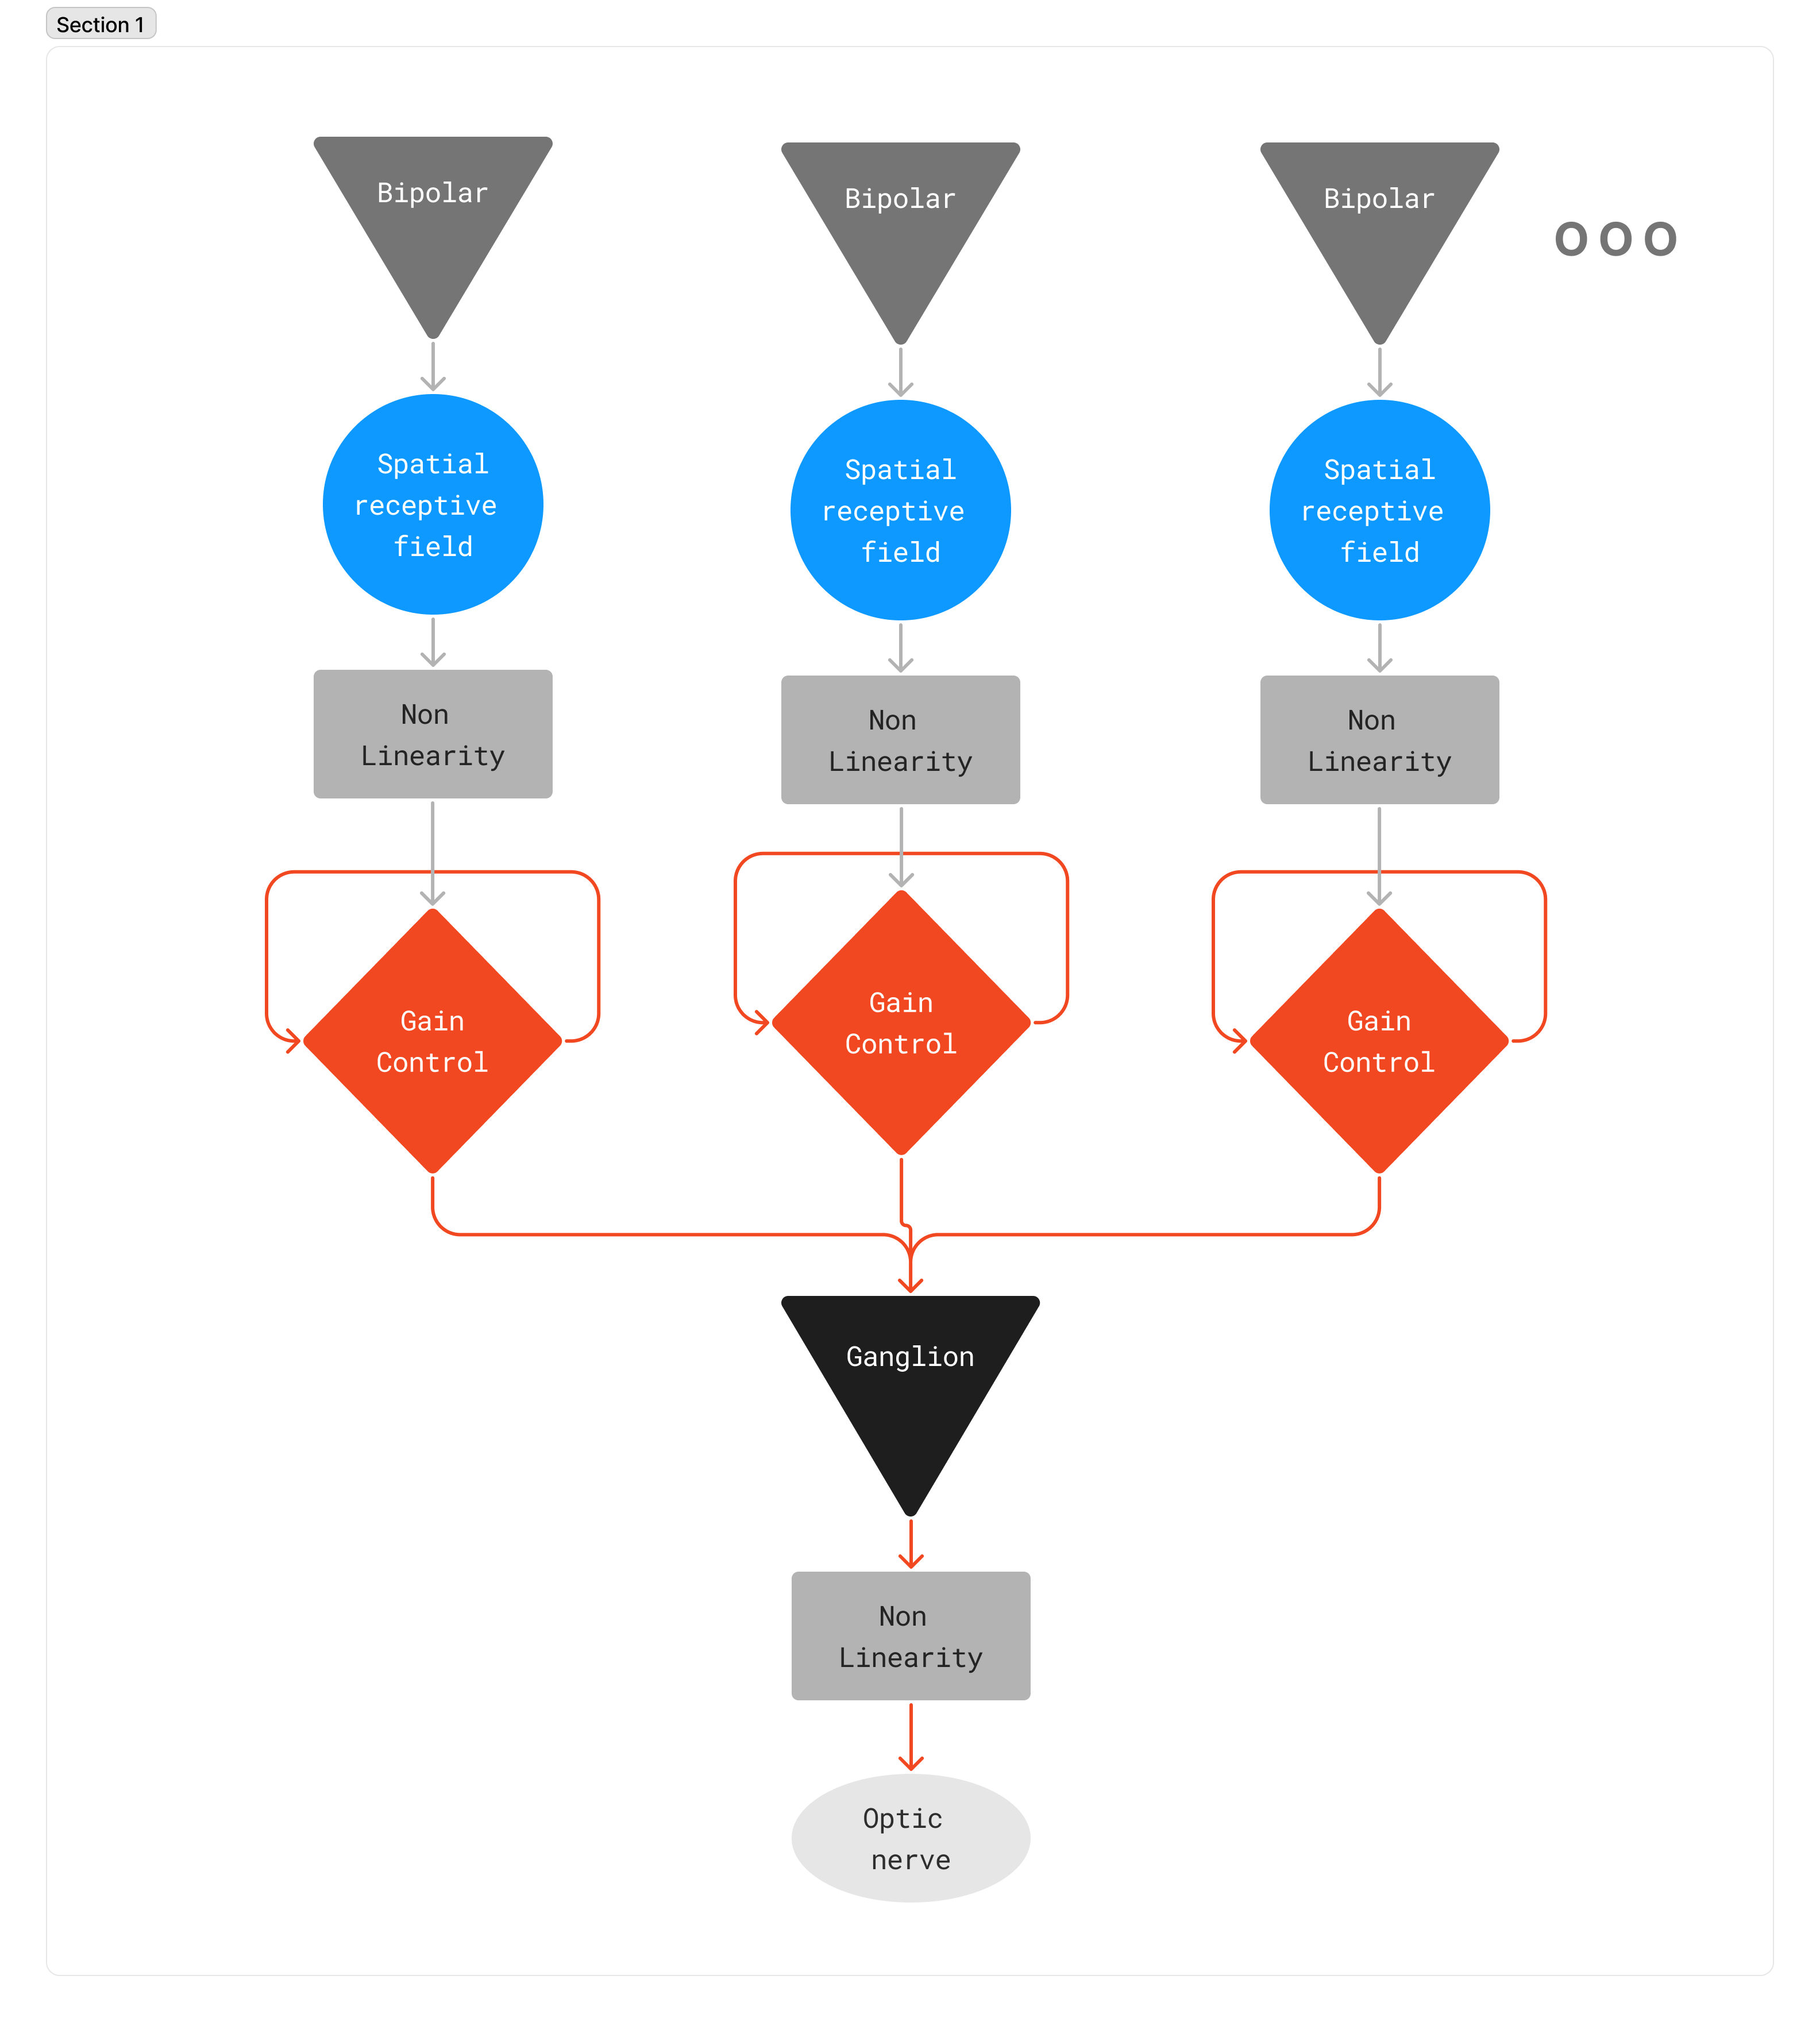
\includegraphics[scale = 0.2]{pics/GCModelDiagram.png}
    \caption{\textbf{Quick sketch of a gain control LNLN model.} Each bipolar
        cell is composed of a linear spatial filter that selectively respond to
        a part
        of the scene, a non-linear activation function, and a gain control
        mechanism
        that scale its output depending on past events. They all converge into
        on
        bipolar cell (forming its own receptive field) of which output is also
        modeled
        using a non-linear function.}\label{fig:LNLN}
\end{figure}
We will first study our models in a data agnostic manner and study its behavior
for different set of parameters. We will then fit it on our own experimental
data using an efficient optimization framework in python using strategies
developed in the field of machine learning.